% I seguenti commenti speciali impostano:
% 1. 
% 2. PDFLaTeX come motore di composizione;
% 3. tesi.tex come documento principale;
% 4. il controllo ortografico italiano per l'editor.

% !TEX encoding = UTF-8
% !TEX TS-program = pdflatex
% !TEX root = tesi.tex
% !TeX spellcheck = <none>

\documentclass[10pt,                    % corpo del font principale
               a4paper,                 % carta A4
               twoside,                 % impagina per fronte-retro
               openright,               % inizio capitoli a destra
               english,                 
               italian,                 
               ]{book}    

\usepackage[utf8]{inputenc}             % codifica di input; anche [latin1] va bene
                                        % NOTA BENE! va accordata con le preferenze dell'editor

%**************************************************************
% Importazione package
%************************************************************** 

%\usepackage{amsmath,amssymb,amsthm}    % matematica

\usepackage[english, italian]{babel}    % per scrivere in italiano e in inglese;
                                        % l'ultima lingua (l'italiano) risulta predefinita

\usepackage{bookmark}                   % segnalibri

\usepackage{caption}                    % didascalie

\usepackage{chngpage,calc}              % centra il frontespizio

\usepackage{csquotes}                   % gestisce automaticamente i caratteri (")

\usepackage{emptypage}                  % pagine vuote senza testatina e piede di pagina

\usepackage{epigraph}					% per epigrafi

\usepackage{eurosym}                    % simbolo dell'euro

\usepackage[T1]{fontenc}                % codifica dei font:
\usepackage{lmodern}                                        % NOTA BENE! richiede una distribuzione *completa* di LaTeX

%\usepackage{indentfirst}               % rientra il primo paragrafo di ogni sezione

\usepackage{graphicx}                   % immagini

\usepackage{hyperref}                   % collegamenti ipertestuali



\usepackage[binding=5mm]{layaureo}      % margini ottimizzati per l'A4; rilegatura di 5 mm

\usepackage{listings}                   % codici

\usepackage{microtype}                  % microtipografia

\usepackage{mparhack,fixltx2e,relsize}  % finezze tipografiche

\usepackage{nameref}                    % visualizza nome dei riferimenti                                      

\usepackage[font=small]{quoting}        % citazioni

\usepackage{subfig}                     % sottofigure, sottotabelle

\usepackage[italian]{varioref}          % riferimenti completi della pagina

\usepackage[dvipsnames,table]{xcolor}         % colori

\usepackage{pgf-pie}
\usepackage{tikz}
\usepackage{pgfplots}
\usepackage{makeidx}
\usepackage{caption}
\usepackage{colortbl}
\usepackage{multirow}
\usepackage{color}
\usepackage{booktabs}                   % tabelle                                       
\usepackage{tabularx}                   % tabelle di larghezza prefissata                                    
\usepackage{longtable}                  % tabelle su più pagine                                        
\usepackage{ltxtable}                   % tabelle su più pagine e adattabili in larghezza

\usepackage[toc, acronym]{glossaries}   % glossario
                                        % per includerlo nel documento bisogna:
                                        % 1. compilare una prima volta tesi.tex;
                                        % 2. eseguire: makeindex -s tesi.ist -t tesi.glg -o tesi.gls tesi.glo
                                        % 3. eseguire: makeindex -s tesi.ist -t tesi.alg -o tesi.acr tesi.acn
                                        % 4. compilare due volte tesi.tex.

\usepackage[backend=biber,style=verbose-ibid,hyperref,backref]{biblatex}
                                        % eccellente pacchetto per la bibliografia; 
                                        % produce uno stile di citazione autore-anno; 
                                        % lo stile "numeric-comp" produce riferimenti numerici
                                        % per includerlo nel documento bisogna:
                                        % 1. compilare una prima volta tesi.tex;
                                        % 2. eseguire: biber tesi
                                        % 3. compilare ancora tesi.tex.

\definecolor{red}{rgb}{1.0, 0.0, 0.0} %http://latexcolor.com/
\definecolor{blue-violet}{rgb}{0.54, 0.17, 0.89}
\definecolor{blush}{rgb}{0.87, 0.36, 0.51}
\definecolor{glaucous}{rgb}{0.38, 0.51, 0.71}
\definecolor{lightcornflowerblue}{rgb}{0.6, 0.81, 0.93}
\definecolor{moonstoneblue}{rgb}{0.45, 0.66, 0.76}
\definecolor{darkcandyapplered}{rgb}{0.64, 0.0, 0.0}
\definecolor{green}{rgb}{0.01, 0.75, 0.24}
\definecolor{coquelicot}{rgb}{1.0, 0.22, 0.0}
\definecolor{dbscan}{HTML}{ABDDD4}
\definecolor{constructCluster}{HTML}{2B83BA}
\definecolor{storeClusterComponent}{rgb}{0.91, 0.41, 0.17}
\definecolor{light-gray}{gray}{0.50}
\definecolor{candyapplered}{rgb}{1.0, 0.03, 0.0}
\definecolor{amber}{rgb}{1.0, 0.75, 0.0}
\definecolor{burntorange}{rgb}{0.8, 0.33, 0.0}
\definecolor{flame}{rgb}{0.89, 0.35, 0.13}
\definecolor{lava}{rgb}{0.81, 0.06, 0.13}
\definecolor{laserlemon}{rgb}{1.0, 1.0, 0.13}
\definecolor{mediumspringgreen}{rgb}{0.0, 0.98, 0.6}
\definecolor{palecopper}{rgb}{0.85, 0.54, 0.4}
\definecolor{alizarin}{rgb}{0.82, 0.1, 0.26}
\definecolor{atomictangerine}{rgb}{1.0, 0.6, 0.4}
\definecolor{ashgrey}{rgb}{0.7, 0.75, 0.71}
\definecolor{beaver}{rgb}{0.62, 0.51, 0.44}
\definecolor{burlywood}{rgb}{0.87, 0.72, 0.53}
\definecolor{cadet}{rgb}{0.33, 0.41, 0.47}
\definecolor{charcoal}{rgb}{0.21, 0.27, 0.31}
\definecolor{darkpastelblue}{rgb}{0.47, 0.62, 0.8}
\definecolor{blue-violet}{rgb}{0.54, 0.17, 0.89}
\definecolor{blush}{rgb}{0.87, 0.36, 0.51}
\definecolor{glaucous}{rgb}{0.38, 0.51, 0.71}
\definecolor{lightcornflowerblue}{rgb}{0.6, 0.81, 0.93}
\definecolor{moonstoneblue}{rgb}{0.45, 0.66, 0.76}




%**************************************************************
% file contenente le impostazioni della tesi
%**************************************************************

%**************************************************************
% Frontespizio
%**************************************************************
\newcommand{\myName}{Andrei Petrov}                                    % autore
\newcommand{\myTitle}{Containerizzazione di Malware Dashboard}                    
\newcommand{\myDegree}{Relazione finale di stage}               % tipo di tesi
\newcommand{\myUni}{Università degli Studi di Padova}           % università
\newcommand{\myFaculty}{Corso di Laurea in Informatica}         % facoltà
\newcommand{\myDepartment}{Dipartimento di Matematica}          % dipartimento
\newcommand{\myProf}{Tullio Vardanega}                          % relatore
\newcommand{\myLocation}{Padova}                                % dove
\newcommand{\myAA}{2016-2017}                                   % anno accademico
\newcommand{\myTime}{ Settembre - 2017}                            % quando


%**************************************************************
% Impostazioni di impaginazione
% see: http://wwwcdf.pd.infn.it/AppuntiLinux/a2547.htm
%**************************************************************

\setlength{\parindent}{14pt} % larghezza rientro della prima riga
\setlength{\parskip}{0pt}    % distanza tra i paragrafi


%**************************************************************
% Impostazioni di biblatex
%**************************************************************
\bibliography{bibliografia} % database di biblatex 

\defbibheading{bibliography}
{
    \cleardoublepage
    \phantomsection 
    \addcontentsline{toc}{chapter}{\bibname}
    \chapter*{\bibname\markboth{\bibname}{\bibname}}
}

\setlength\bibitemsep{1.5\itemsep} % spazio tra entry

\DeclareBibliographyCategory{opere}
\DeclareBibliographyCategory{web}

\addtocategory{opere}{womak:lean-thinking}
\addtocategory{opere}{baier:getting-started-k8s}
\addtocategory{opere}{vohra:k8s-micro-docker}
\addtocategory{opere}{turnbull:docker-book}
\addtocategory{opere}{gormlery:es}
\addtocategory{opere}{kuc:es}

\addtocategory{web}{site:k8s}
\addtocategory{web}{site:docker}
\addtocategory{web}{site:es}
\addtocategory{web}{site:logstash}
\addtocategory{web}{site:kibana}
\addtocategory{web}{site:nginx}
\addtocategory{web}{site:linux}
\addtocategory{web}{site:micro}
\addtocategory{web}{site:micro-fawler}
\addtocategory{web}{site:micro-wiki}
\addtocategory{web}{site:cloud-wiki}

\defbibheading{opere}{\section*{Bibliografia}}
\defbibheading{web}{\section*{Sitografia}}


%**************************************************************
% Impostazioni di caption
%**************************************************************
\captionsetup{
    tableposition=top,
    figureposition=bottom,
    font=small,
    format=hang,
    labelfont=bf
}

%**************************************************************
% Impostazioni di glossaries
%**************************************************************

%**************************************************************
% Acronimi
%**************************************************************
\renewcommand{\acronymname}{Acronimi e abbreviazioni}

\newacronym[description={\glslink{apig}{Application Program Interface}}]
    {api}{API}{Application Program Interface}


\newacronym[description={\glslink{iksg}{Information and Knowledge Supply}}]
	{iks}{IKS}{Information and Knowledge Supply}

\newacronym[description={\glslink{ictg}{Information and Communication Technology}}]
	{ict}{ICT}{Information and Communication Technology}

\newacronym[description={\glslink{itg}{Information Technology}}]
	{it}{IT}{Information Technology}


%**************************************************************
% Glossario
%**************************************************************
\renewcommand{\glossaryname}{Glossario}

\newglossaryentry{framework}{
	name=\glslink{framework}{Framework},
	text=Framework,
	sort=framework,
	description={Architettura logica di supporto su cui un software
		può essere progettato e realizzato, spesso facilitandone lo sviluppo da parte del
		programmatore. La sua funzione è quella di creare una infrastruttura generale,
		lasciando al programmatore il contenuto vero e proprio dell’applicazione.
		}
}


\newglossaryentry{patching}{
	name=\glslink{patching}{Patching},
	text=Patching,
	sort=patching,
	description={
	Applicare una patch, porzione di software progettata per aggiornare o migliorare un programma. Una patch permette di risolvere vulnerabilità di sicurezza e altri BugFix di un applicativo sviluppato.
	}
}
\newglossaryentry{agile}{
	name=\glslink{agile}{Agile},
	text=Agile (metodologia),
	sort=agile,
	description={
	Metodo per lo sviluppo del software che coinvolge quanto pi`u possibile il committente, ottenendo in tal modo una elevata reattivit`a alle sue richieste.
	}
}
\newglossaryentry{repository}{
	name=\glslink{repository}{Repository},
	text=Repository,
	sort=repository,
	description={
	Ambiente di un sistema informativo, in cui vengono gestiti
	i metadati, attraverso tabelle relazionali; l’insieme di tabelle, regole e motori
	di calcolo tramite cui si gestiscono i metadati prende il nome di metabase.
	}
}
\newglossaryentry{deployment}{
	name=\glslink{deployment}{Deployment},
	text=Deployment,
	sort=deployment,
	description={
	Consegna o rilascio al cliente, con relativa installazione e messa
	in funzione o esercizio, di una applicazione o di un sistema software tipicamente
	all’interno di un sistema informatico aziendale.
	}
}

\newglossaryentry{cloud}{
	name=\glslink{cloud}{Cloud},
	text=Cloud,
	sort=cloud,
	description={
	Paradigma di erogazione di risorse informatiche, come
	l’archiviazione, l’elaborazione o la trasmissione di dati, caratterizzato dalla
	disponibilità on demand attraverso Internet a partire da un insieme di risorse
	preesistenti e configurabili.
	}
}
%\newglossaryentry{}
%\newglossaryentry{}
%\newglossaryentry{}
%\newglossaryentry{}
%\newglossaryentry{}
%\newglossaryentry{}
%\newglossaryentry{}

\newglossaryentry{apig}
{
    name=\glslink{api}{API},
    text=Application Program Interface,
    sort=api,
    description={Il termine \emph{Application Programming Interface API} (ing. interfaccia di programmazione di un'applicazione) si indica ogni insieme di procedure disponibili al programmatore, di solito raggruppate a formare un set di strumenti specifici per l'espletamento di un determinato compito all'interno di un certo programma. La finalità è ottenere un'astrazione, di solito tra l'hardware e il programmatore o tra software a basso e quello ad alto livello semplificando così il lavoro di programmazione}
}

\newglossaryentry{ictg}
{
	name=\glslink{ict}{ICT},
	text=Information and Communication Technology,
	sort=ict,
	description={insieme di metodi e tecnologie che implementano i sistemi di trasmissione, ricezione e elaborazione di informazioni.}
}

\newglossaryentry{itg}
{
	name=\glslink{it}{IT},
	text=Information Technology,
	sort=it,
	description={utilizzo di qualsiasi tecnologia di calcolo per offrire servizio di memorizzazione, reti per creare, processare, memorizzare e mettere in sicurezza ogni forma immaginabile di dato elettronico.
    }
}



\newglossaryentry{private equity}{
	name=\glslink{private equity}{Private equity},
	text=Private equity,
	sort=private,
	description={
	Da definire
	}
}

\newglossaryentry{IKS}{
	name=\glslink{iks}{IKS},
	text=IKS,
	sort=iks,
	description={
		IL nome dell'azienda è un acronimo inglese che ne determina lo spirito e la filosofia. 
	}
}

 % database di termini
\makeglossaries


%**************************************************************
% Impostazioni di graphicx
%**************************************************************
\graphicspath{{immagini/}} % cartella dove sono riposte le immagini


%**************************************************************
% Impostazioni di hyperref
%**************************************************************
\hypersetup{
    %hyperfootnotes=false,
    %pdfpagelabels,
    %draft,	% = elimina tutti i link (utile per stampe in bianco e nero)
    colorlinks=true,
    linktocpage=true,
    pdfstartpage=1,
    pdfstartview=FitV,
    % decommenta la riga seguente per avere link in nero (per esempio per la stampa in bianco e nero)
    %colorlinks=false, linktocpage=false, pdfborder={0 0 0}, pdfstartpage=1, pdfstartview=FitV,
    breaklinks=true,
    pdfpagemode=UseNone,
    pageanchor=true,
    pdfpagemode=UseOutlines,
    plainpages=false,
    bookmarksnumbered,
    bookmarksopen=true,
    bookmarksopenlevel=1,
    hypertexnames=true,
    pdfhighlight=/O,
    %nesting=true,
    %frenchlinks,
    urlcolor=webbrown,
    linkcolor=RoyalBlue,
    citecolor=webgreen,
    %pagecolor=RoyalBlue,
    %urlcolor=Black, linkcolor=Black, citecolor=Black, %pagecolor=Black,
    pdftitle={\myTitle},
    pdfauthor={\textcopyright\ \myName, \myUni, \myFaculty},
    pdfsubject={},
    pdfkeywords={},
    pdfcreator={pdfLaTeX},
    pdfproducer={LaTeX}
}

%**************************************************************
% Impostazioni di itemize
%**************************************************************
\renewcommand{\labelitemi}{$\ast$}

%\renewcommand{\labelitemi}{$\bullet$}
%\renewcommand{\labelitemii}{$\cdot$}
%\renewcommand{\labelitemiii}{$\diamond$}
%\renewcommand{\labelitemiv}{$\ast$}


%**************************************************************
% Impostazioni di listings
%**************************************************************
\lstset{
    language=[LaTeX]Tex,%C++,
    keywordstyle=\color{RoyalBlue}, %\bfseries,
    basicstyle=\small\ttfamily,
    %identifierstyle=\color{NavyBlue},
    commentstyle=\color{Green}\ttfamily,
    stringstyle=\rmfamily,
    numbers=none, %left,%
    numberstyle=\scriptsize, %\tiny
    stepnumber=5,
    numbersep=8pt,
    showstringspaces=false,
    breaklines=true,
    frameround=ftff,
    frame=single
} 


%**************************************************************
% Impostazioni di xcolor
%**************************************************************
\definecolor{webgreen}{rgb}{0,.5,0}
\definecolor{webbrown}{rgb}{.6,0,0}


%**************************************************************
% Altro
%**************************************************************

\newcommand{\omissis}{[\dots\negthinspace]} % produce [...]

% eccezioni all'algoritmo di sillabazione
\hyphenation
{
    ma-cro-istru-zio-ne
    gi-ral-din
}

\newcommand{\sectionname}{sezione}
\addto\captionsitalian{\renewcommand{\figurename}{Figura}
                       \renewcommand{\tablename}{Tabella}}

\newcommand{\glsfirstoccur}{\ap{{[g]}}}

\newcommand{\intro}[1]{\emph{\textsf{#1}}}

%**************************************************************
% Environment per ``rischi''
%**************************************************************
\newcounter{riskcounter}                % define a counter
\setcounter{riskcounter}{0}             % set the counter to some initial value

%%%% Parameters
% #1: Title
\newenvironment{risk}[1]{
    \refstepcounter{riskcounter}        % increment counter
    \par \noindent                      % start new paragraph
    \textbf{\arabic{riskcounter}. #1}   % display the title before the 
                                        % content of the environment is displayed 
}{
    \par\medskip
}

\newcommand{\riskname}{Rischio}

\newcommand{\riskdescription}[1]{\textbf{\\Descrizione:} #1.}

\newcommand{\risksolution}[1]{\textbf{\\Soluzione:} #1.}

%**************************************************************
% Environment per ``use case''
%**************************************************************
\newcounter{usecasecounter}             % define a counter
\setcounter{usecasecounter}{0}          % set the counter to some initial value

%%%% Parameters
% #1: ID
% #2: Nome
\newenvironment{usecase}[2]{
    \renewcommand{\theusecasecounter}{\usecasename #1}  % this is where the display of 
                                                        % the counter is overwritten/modified
    \refstepcounter{usecasecounter}             % increment counter
    \vspace{10pt}
    \par \noindent                              % start new paragraph
    {\large \textbf{\usecasename #1: #2}}       % display the title before the 
                                                % content of the environment is displayed 
    \medskip
}{
    \medskip
}

\newcommand{\usecasename}{UC}

\newcommand{\usecaseactors}[1]{\textbf{\\Attori Principali:} #1. \vspace{4pt}}
\newcommand{\usecasepre}[1]{\textbf{\\Precondizioni:} #1. \vspace{4pt}}
\newcommand{\usecasedesc}[1]{\textbf{\\Descrizione:} #1. \vspace{4pt}}
\newcommand{\usecasepost}[1]{\textbf{\\Postcondizioni:} #1. \vspace{4pt}}
\newcommand{\usecasealt}[1]{\textbf{\\Scenario Alternativo:} #1. \vspace{4pt}}

%**************************************************************
% Environment per ``namespace description''
%**************************************************************

\newenvironment{namespacedesc}{
    \vspace{10pt}
    \par \noindent                              % start new paragraph
    \begin{description} 
}{
    \end{description}
    \medskip
}

\newcommand{\classdesc}[2]{\item[\textbf{#1:}] #2}                     % file con le impostazioni personali

\begin{document}
%**************************************************************
% Materiale iniziale
%**************************************************************
\frontmatter
% !TEX encoding = UTF-8
% !TEX TS-program = pdflatex
% !TEX root = ../tesi.tex
% !TeX spellcheck = de_DE

%**************************************************************
% Frontespizio 
%**************************************************************
\begin{titlepage}

\begin{center}

\begin{LARGE}
\textbf{\myUni}\\
\end{LARGE}

\vspace{10pt}

\begin{Large}
\textsc{\myDepartment}\\
\end{Large}

\vspace{10pt}

\begin{large}
\textsc{\myFaculty}\\
\end{large}

\vspace{30pt}
\begin{figure}[htbp]
\begin{center}

\includegraphics[height=6cm]{logo-unipd}
\end{center}
\end{figure}
\vspace{30pt} 

\begin{LARGE}
\begin{center}
\textbf{\myTitle}\\
\end{center}
\end{LARGE}

\vspace{10pt} 

\begin{large}
\textsl{\myDegree}\\
\end{large}

\vspace{40pt} 

\begin{large}
\begin{flushleft}
\textit{Relatore}\\ 
\vspace{5pt} 
Prof. \myProf
\end{flushleft}

\vspace{0pt} 

\begin{flushright}
\textit{Laureando}\\ 
\vspace{5pt} 
\myName
\end{flushright}
\end{large}

\vspace{40pt}

\line(1, 0){338} \\
\begin{normalsize}
\textsc{Anno Accademico \myAA}
\end{normalsize}

\end{center}
\end{titlepage} 
% !TEX encoding = UTF-8
% !TEX TS-program = pdflatex
% !TEX root = ../tesi.tex
% !TeX spellcheck = de_DE

%**************************************************************
% Colophon
%**************************************************************
\clearpage
\phantomsection
\thispagestyle{empty}

\hfill

\vfill

\noindent\myName: \textit{\myTitle,}
\myDegree,
\textcopyright\ \myTime.
% !TEX encoding = UTF-8
% !TEX TS-program = pdflatex
% !TEX root = ../tesi.tex
% !TeX spellcheck = de_DE

%**************************************************************
% Sommario
%**************************************************************
\cleardoublepage
\phantomsection
\pdfbookmark{Sommario}{Sommario}
\begingroup
\let\clearpage\relax
\let\cleardoublepage\relax
\let\cleardoublepage\relax

\chapter*{Sommario}

//TODO

%\vfill
%
%\selectlanguage{english}
%\pdfbookmark{Abstract}{Abstract}
%\chapter*{Abstract}
%
%\selectlanguage{italian}

\endgroup			

\vfill


% !TEX encoding = UTF-8
% !TEX TS-program = pdflatex
% !TEX root = ../tesi.tex
% !TeX spellcheck = de_DE

%**************************************************************
% Indici
%**************************************************************
\cleardoublepage
\pdfbookmark{\contentsname}{tableofcontents}
\setcounter{tocdepth}{4}
\setcounter{secnumdepth}{4}
\tableofcontents
%\markboth{\contentsname}{\contentsname} 
\clearpage

\begingroup 
    \let\clearpage\relax
    \let\cleardoublepage\relax
    \let\cleardoublepage\relax
    %*******************************************************
    % Elenco delle figure
    %*******************************************************    
    \phantomsection
    \pdfbookmark{\listfigurename}{lof}
    \listoffigures

    \vspace*{8ex}

    %*******************************************************
    % Elenco delle tabelle
    %*******************************************************
    \phantomsection
    \pdfbookmark{\listtablename}{lot}
    \listoftables
        
    \vspace*{8ex}
\endgroup

\cleardoublepage

\cleardoublepage

%**************************************************************
% Materiale principale
%**************************************************************
\mainmatter
% !TEX encoding = UTF-8
% !TEX TS-program = pdflatex
% !TEX root = ../tesi.tex
% !TEX spellcheck = it-IT

%**************************************************************
\chapter{L'Azienda}
\label{cap:azienda}
\vspace{20pt}

\section{IKS}

IKS \emph{(Information Knowledge. Supply)} è un'azienda padovana 
fondata, dall'attuale Amministratore Delegato Paolo Pittarello, nel 1999. 

Nell'insieme, IKS unisce figure di alto profilo con lo scopo di 
proporre soluzioni innovative alle richieste di mercato dell'\gls{ict} 
sia italiano che estero. Le soluzioni offerte interessano in particolare 
gli ambiti della sicurezza, dell'infrastruttura e della governance \gls{it}.  

L'azienda è in continua ricerca tecnologica. Investendo sulla formazione 
del proprio personale, IKS si impegna di portare solo valore aggiunto 
al business dei propri clienti. Inoltre, l'Azienda crede fortemente 
nell'innovazione come strumento verso un ambiente digitale comune, 
\gls{agile} e totalmente disponibile. 

Il quartier generale aziendale è a Padova. Inoltre, IKS possiede uffici 
anche nelle seguenti città: Roma, Milano e Trento.

A partire dallo scorso anno (2016), IKS SRL, Kirey SRL, Insirio SPA e 
System Evolution SRL hanno  fondato il Gruppo Kirey. L'obiettivo comune 
delle quattro aziende è l'unione delle competenze complementari e 
garantire un portfolio completo di soluzioni ai clienti attuali e futuri. 

La creazione del Gruppo Kirey è stata guidata dalla Synergo SGR., società di 
\emph{private equity}. Il presidente del nuovo Gruppo commerciale è Vittorio 
Lusvarghi.   

A seguito della creazione del Gruppo, IKS SRL e le restanti tre realtà 
aziendali hanno conservato la propria struttura di governance e management, 
con il fine di garantire la propria continuità gestionale. 

\section{Profilo dell'azienda}
\subsection{Servizi e prodotti offerti}

Nel corso degli anni, IKS si è fatta notare per gli enormi contributi 
innovativi nell'ambito della sicurezza informatica. Tuttavia, essa non 
è limitata a questo ambito. Infatti, gli altri ambiti di applicazione 
sono: infrastruttura e governance IT. 

Di seguito vengono presentati i servizi offerti da IKS per ciascun ambito di 
applicazione:

\begin{itemize}
	\item \textbf{IT Security}\\
	 \begin{itemize}
	 	\item \textbf{Risk analysis e vulnerability assessment}\\ 
	 	È importante garantire la sicurezza dell'infrastruttura 
		informatica nel suo complesso. A questo scopo, IKS offre un 
		servizio orientato alla ricerca di eventuali vulnerabilità e 
		analisi dei rischi a esse collegate;
	 
	 	\begin{figure}[htbp]
	 		\begin{center}
	 			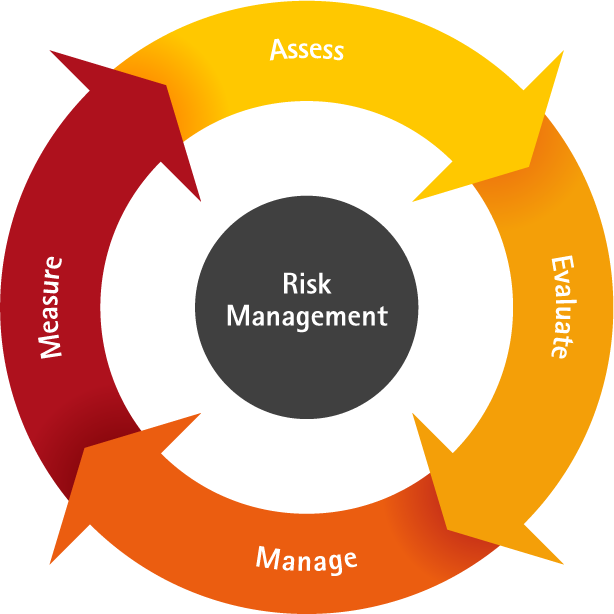
\includegraphics[height=4cm]{risk-management}
	 			\caption{Visione a processo della gestione del 
				 rischio.Immagine tratta da: http://bit.ly/2rh3V0A.}
	 		\end{center}
	 	\end{figure}
	 		 	
		\item \textbf{Audit management}\\
		Le aziende di continuo sono sottoposte a controlli di vario 
		genere; il loro scopo è l'accertamento della 
		regolarità delle aziende con: certificazioni, normative, bilanci 
		ed ecc. IKS offre un servizio di supporto per le aziende con 
		il fine di agevolare le attività di \emph{auditing} 
		ed eventualmente per migliorare i loro processi interni;
		\begin{figure}[htbp]
			\begin{center}
				\hspace{3em}
				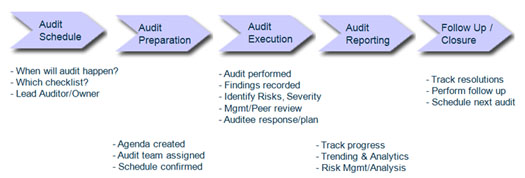
\includegraphics[height=3.5cm]{audit-management}
				\caption{Flusso di lavoro durante lo 
				svolgimento di un \emph{audit}.
				Immagine tratta da: http://bit.ly/2rdFhfv.}
			\end{center}
		\end{figure}
	
	 	\item \textbf{Difesa perimetrale}\\ 
	 	Sempre in ambito della sicurezza è importante prendere le 
		giuste misure per garantire a priori uno specifico livello 
		di sicurezza e limitare a zero le intrusioni dall'esterno 
	 	di un'infrastruttura IT aziendale. A questo scopo, IKS offre 
		un'insieme di soluzioni orientare al monitoraggio degli 
		accessi a sistemi aziendali, dei permessi sulle operazioni 
	 	che un utente può effettuare, e molto altro;
	 	\begin{figure}[htbp]
	 		\begin{center}
	 			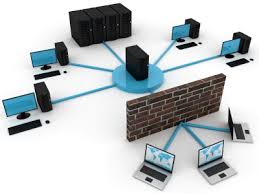
\includegraphics[height=4cm]{firewall}
	 			\caption{Visione grafica del concetto di difesa 
				perimetrale. Immagine tratta da: 
				http://bit.ly/2s834O2.}
	 		\end{center}
	 	\end{figure}	 	
	 \end{itemize}	
	\item \textbf{IT Infrastructure}\\
	 \begin{itemize}
	 	\item \textbf{Business continuity}\\
	 	In ambito bancario, le infrastrutture informatiche sono molto 
		complesse. La manutenzione delle infrastrutture informatiche non è 
		semplice. La sfida più difficile è garantire che questi sistemi siano 
		operativi al 100\%. Una simile percentuale nella pratica è 
		impossibile. IKS con il proprio gruppo di esperti sono alla 
		continua ricerca di soluzioni per incrementare la percentuale 
		di continuità operativa di questi sistemi. Infatti, le 
		soluzioni offerte dall'azienda sono orientate nel concreto 
		all'infrastruttura del cliente richiedente supporto;
	 	\begin{figure}[htbp]
	 		\begin{center}
	 		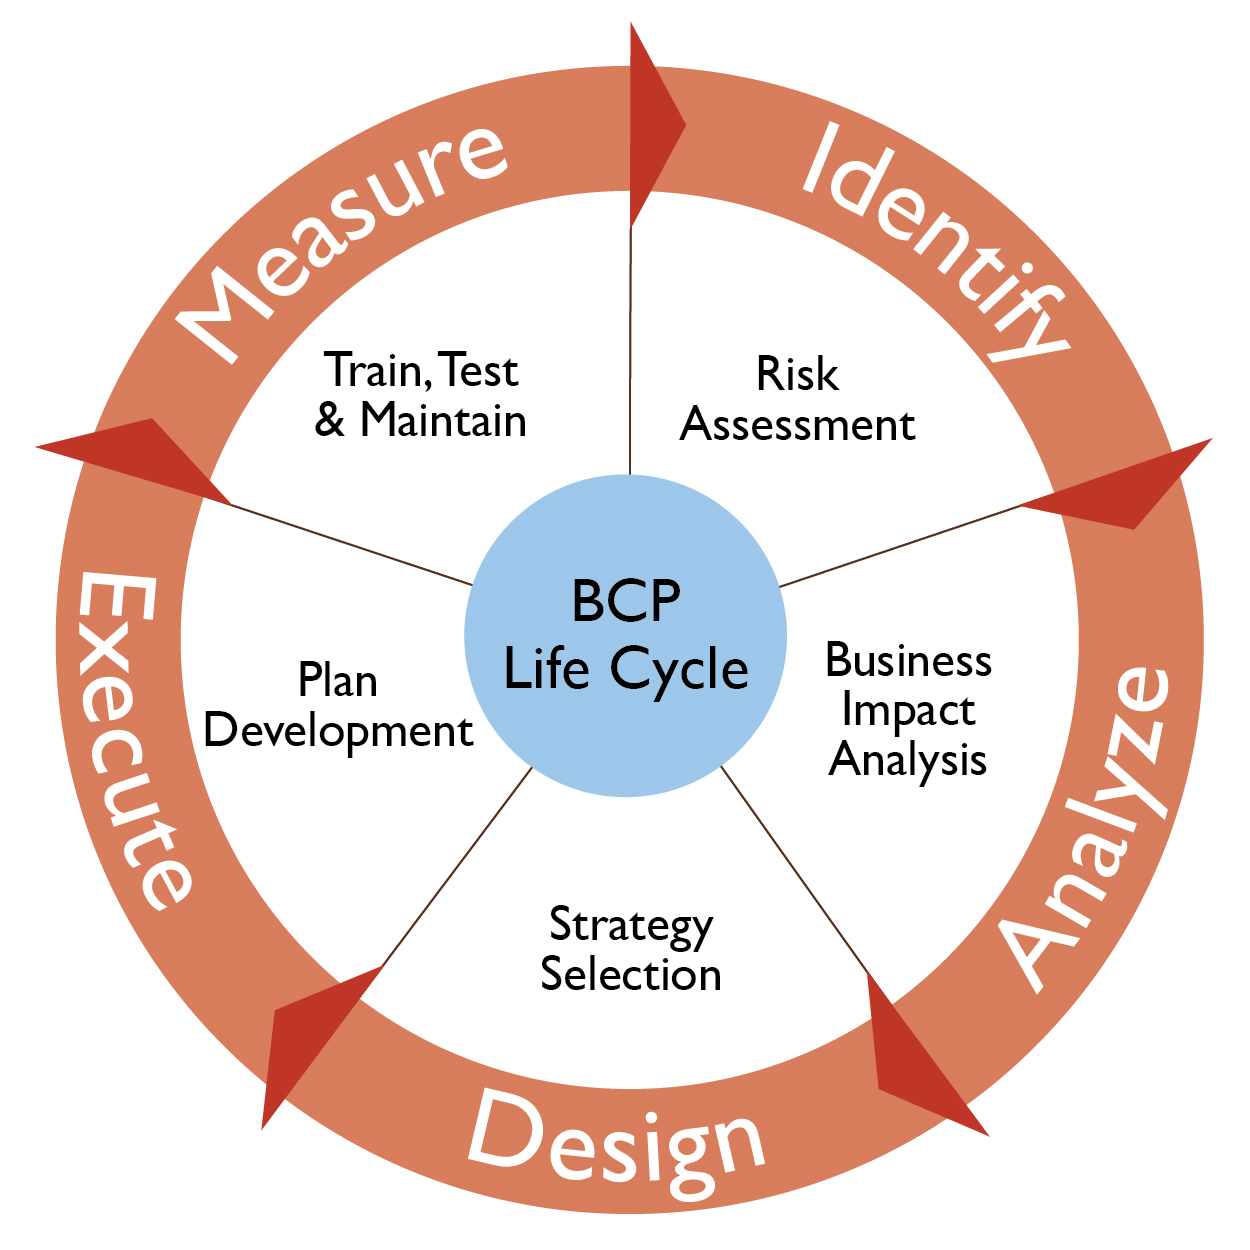
\includegraphics[height=5cm]{business-continuity}
				\caption{Visione del ciclo di vita del 
				processo di \emph{business continuity}. 
				Immagine tratta da: http://bit.ly/2qvCmgP.}
			\end{center}
			\end{figure}

%\newpage
		\item \textbf{Virtualization technology}\\
		 Ogni prodotto software di business per portare valore aggiunto 
		 deve essere eseguito. Eseguire un prodotto software per server 
		 fisico richiede la disponibilità di un cospicuo numero di server. 
		 A questo scopo la tecnologia di virtualizzazione permette la 
		 creazione di server virtuali che eseguono programmi e questi 
		 vengono eseguiti da server fisici. I benefici di una simile 
		 infrastruttura è l'ottimizzazione delle risorse di calcolo, 
		 agilità di gestione e sicurezza. Alcune delle soluzioni di 
		 virtualizzazione offerte da IKS sono: VMWare, RHEV ed ecc. 
		 Un'evoluzione della tecnologia di virtualizzazione è il \emph{Cloud}. 
		 In questo ambito, IKS propone soluzioni di migrazione e supporto 
		 verso il Cloud dell'infrastruttura IT classica di un'azienda;  
		 \begin{figure}[htbp]
			\begin{center}
				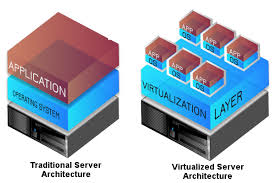
\includegraphics[height=4cm]{virtualization}
				\caption{Vista a confronto: ambiente 
				server bare metal e virtualizzato. 
				Immagine tratta da: http://bit.ly/2qvtLLk.}
			\end{center}
		 \end{figure}
 	\end{itemize}

	\item \textbf{IT Governance}\\
	\begin{itemize}
		\item \textbf{Service management}\\
		Un servizio informatico di business, a causa della sua criticità,
		richiede costante attenzione. Il monitoraggio del servizio 
		informatico presenta la necessità di enormi investimenti 
		economici. IKS offre piani di gestione per soddisfare 
		anche i più esigenti clienti;
	    
	    \begin{figure}[htbp]
	    	\begin{center}
	    		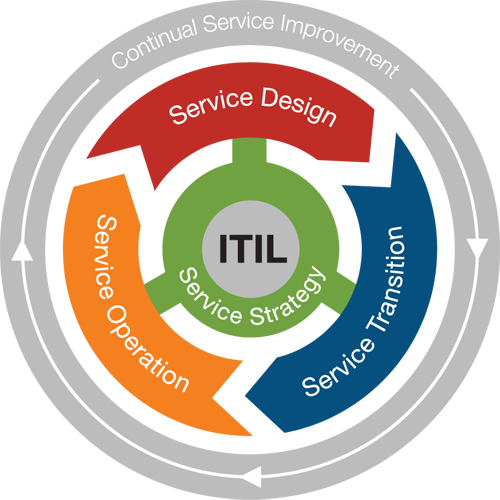
\includegraphics[height=5cm]{itil}
	    		\caption{Visione della gestione di servizio in 
				prospettiva del \gls{framework} ITIL. Immagine tratta da: 
				http://bit.ly/2qvNryk.}
	    	\end{center}
	    \end{figure}
	    
		\item \textbf{Application and performance monitoring}\\ 
		Ogni prodotto software ha il proprio specifico ciclo di vita. 
		Concluso il ciclo di sviluppo, il prodotto è rilasciato in 
		produzione. La seconda parte del ciclo di vita di un prodotto 
		software è la manutenzione. Il monitoraggio di un applicativo 
		è importante per avere una costante visione dello stato del 
		prodotto e prevenire eventuali esigenze di manutenzione generica 
		oppure di basso profilo a livello di codice sorgente. In questo 
		dominio, grazie a partnership strategiche, IKS offre soluzioni 
		mirate a garantire la miglior possibile esperienza di 
		monitoraggio applicativo;
		
		\item \textbf{System and networking management}\\
		Gestire sistemi e reti informatiche è un compito complesso. 
		L'utilizzo di strumenti adeguati permette di semplificare il 
		lavoro e garantisce un stato consistente del sistema nel tempo. 
		Le soluzioni che IKS offre sono orientate alla flessibilità e 
		facilità d'uso dei prodotti offerti in questo contesto;
	\end{itemize} 
	\item \textbf{Innovation \& Project} \\
	\begin{itemize}
		\item \textbf{Architetture applicative distribuite}\\
		I sistemi informatici diventano sempre più di natura 
		distribuita. IKS offre in questo ambito soluzioni architetturali 
		orientate a microservizi, utilizzando le ultime tecnologie 
		orientate alla containerizzazione e orchestrazione di container; 
		
		\item \textbf{Sviluppo di applicazioni cloud native}\\
		È comune sentire parlare di cloud. Le classiche 
        architetture applicative non riescono a beneficiare della 
		flessibilità del cloud, perché in organizzazione e struttura 
		non sono scalabili e sono difficilmente modularizzabili. Applicazioni
		che vengono gestite nel complesso come un'unica unità prendono il nome di 
		monolite. La diretta conseguenza di una simile organizzazione è 
		il carattere statico e poco flessibile dell'applicazione. Paradigmi nuovi, 
		per la messa in esercizio di applicazioni, mancano l'intigrazione 
		con architetture software tradizionali. Per questo motivO, 
		le applicazioni devono essere sviluppate fin dal principio con 
		un'architettura orientata al Cloud. Una buona guida, di sviluppo 
		di applicazioni orientate al Cloud, è la segeunte: \textit{Twelve Factor-Factor App}.,
		Heroku, servizio  PaaS per applicazioni cloud native, promuove 
		continuamente l'importanza dei 12 principi alla base della filosofia 
		\emph{cloud native}. In questa direzione IKS propone servizi di sviluppo 
		di applicazioni di business orientate all'affidabilità, resilienza, 
		scalabilità orizzontale ed ecc.
		
		\begin{figure}[htbp]
			\begin{center}		
			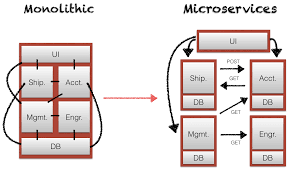
\includegraphics[height=5cm]{monolith-microservice}
			\caption{Visione architetturale a monolite e 
				microservizi a confronto. 
				Immagine tratta da: http://bit.ly/2rh1niY.}
			\end{center}
			\end{figure}
			\end{itemize} 
		\end{itemize}

La clientela tipica di IKS sono le aziende operanti nei seguenti ambiti: 
pubblica amministrazione, bancario, assicurativo e servizi. 

Una lista dettagliata delle referenze può essere consultata sul sito
di IKS (\url{https://www.iks.it/referenze.html}).

\subsection{Struttura organizzativa}

Ad oggi, IKS conta più di 100 dipendenti. La sua organizzazione interna è 
riassunta nel diagramma in \textbf{Figura 1.8}.

In seguito, descrivo le unità operative che costituiscono il nucleo 
decisionale dell'azienda. Queste unità sono:
\begin{itemize}
	\item \textbf{Direzione}\\ 
	Definisce gli orientamenti e le politiche aziendali, gli 
	obiettivi per la qualità, riesamina periodicamente il sistema di 
	qualità e gestisce il piano di formazione dei dipendenti in funzione 
	alle esigenze e motivazioni personali;
	\item \textbf{Direzione Commerciale}\\
	Definisce le politiche commerciali, gli obiettivi e le risorse 
	necessarie. Promuove i servizi e prodotti dell'azienda. Gestisce i 
	clienti, i fornitori e le offerte contrattuali;
	\item \textbf{Direzione tecnica o Operation}\\
	Supporta la Direzione Commerciale nella valutazione commerciale di 
	prodotti e/o offerte dal punti di vista tecnico. Gestisce a livello 
	tecnico i progetti e servizi. Pianifica le risorse necessarie per 
	i prodotti/servizi. Verifica lo stato del prodotto/servizio offerto;	
	\item \textbf{Amministrazione \& Finanza}\\
	Gestisce la documentazione di progetto, su coordinamento della direzione 
	commerciale e tecnica. Gestisce l'archiviazione della documentazione;
	\item \textbf{Acquisti}\\
	Su coordinamento della Direzione, gestisce i fornitori di prodotti e 
	servizi. Gestisce il processo di acquisizione di nuovi prodotti o 
	servizi. Il processo di acquisizione è guidato dalle necessità 
	interne aziendali oppure da quelle dei clienti;
	\item \textbf{Assicurazione Qualità}\\
	È a stretto contatto solo con la Direzione. Gestisce il piano di 
    qualità, coordina le attività di ispezione, misura e stima il livello 
	della qualità aziendale;
	\item \textbf{Business Unit (BU)}\\
	Gestisce i progetti o servizi concordati con il Cliente. Rendiconta 
	direttamente alla Direzione Tecnica e gestisce l'emissione delle 
	fatture verso il Cliente. 
\end{itemize}


\begin{figure}[htbp]
	\begin{center}
		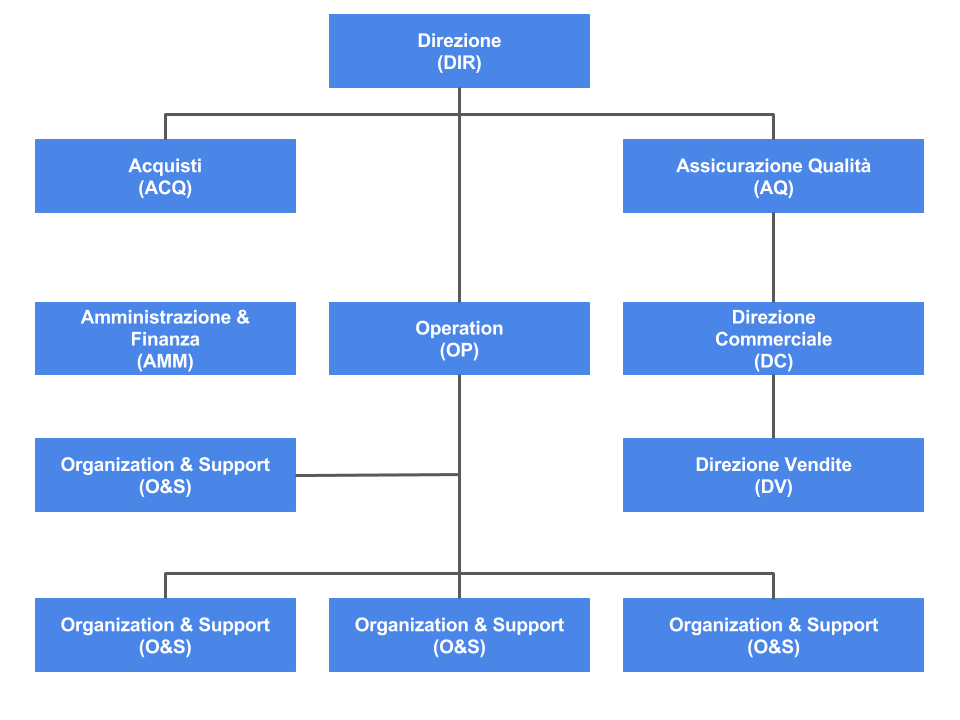
\includegraphics[height=8cm]{organigramma}
		\caption{Organigramma aziendale}
	\end{center}
\end{figure}



\subsection{Processi aziendali}

IKS, a partire dal 2003, è certificata UNI EN ISO 9001. Questo certifica che 
l'azienda cura molto la qualità del proprio lavoro. Infatti, il miglioramento 
continuo permette all'azienda di rimanere competitiva e consolidare 
la propria posizione di leader sul mercato del ICT italiano. Riporto, di seguito, 
alcuni obiettivi di qualità dell'azienda:

\begin{itemize}
	\item Mantenere e aumentare il livello di soddisfazione del Cliente;
	\item Operare in modo efficiente ed efficace per soddisfare i requisiti 
		  contrattuali, norme e regolamenti;
	\item Monitorare i propri processi per: garantire azioni correttive 
	      tempestivamente e permettere un comportamento pro attivo, 
	      anticipare i bisogni e predire le risorse aziendali necessarie 
	      prima dell'effettivo bisogno; 
	\item Assicurare una adeguata formazione al Personale.
\end{itemize}


Il Cliente copre un ruolo importante nella quotidinità di IKS. Infatti, 
l'azienda cerca di coinvolgere i propri clienti il più possibile., questo 
è necessario per comprendere meglio i bisogni attuali del cliente e 
cogliere esigenze future. 
In azienda, il passo successivo alla formalizzazione del bisogno del 
Cliente segue un'attività di analisi dei requisiti. L'obiettivo 
dell'attività è la dettagliata comprensione del contesto applicativo, 
quali sono le parti interagenti e quali possono essere i rischi, durante 
l'attività di progetto, per implementare i bisogni del Cliente.

A progetto concluso, il Cliente valuta criticamente la soluzione 
presentata. La valutazione, eventualmente, coinvolge un reclamo. Questo 
è rivolto alla Direzione dell'Azienda.

IKS organizza il proprio lavoro per processi: primari, direttivi e di supporto. 
Ciascuna categoria di processo definisce delle responsabilità e compiti. 
Per esempio, i processi organizzativi interessano le attività per: definire la politica 
e strategia aziendale, pianificare e allocare le risorse, riesaminare la gestione del 
sistema di qualità. Invece, i processi primari ricoprono attività che garantiscono 
un diretto ricavo economico per l'azienda e danno un valore aggiunto al prodotto o 
servizio fornito. Esempi di attività in questa categoria sono: proporre offerte 
commerciali ai clienti, progettare e sviluppare prodotti software, erogare servizi IT. 
L'ultima categoria di processi sono i processi di supporto. Le consone attività giornaliere 
riguardano: gestire le risorse umane, l'infrastruttura 
e gli ambienti di lavoro., monitorare e analizzare la qualità aziendale. 

In \textbf{Figura 1.9} segue una presentazione dello schema organizzativo 
utilizzato dall'Azienda, durante il ciclo di vita di un progetto.

Periodicamente, il responsabile della qualità, incaricato della Direzione, attua 
attività d'ispezione. L'obiettivo dell'attività è il controllo del livello di qualità
fornita dai dipendenti aziendali. A posteriori, segue un'attività di 
analisi e misura dei livelli di qualità organizzati per BU, servizio e 
prodotto offerto da IKS.

\begin{figure}[htbp]
	\begin{center}
		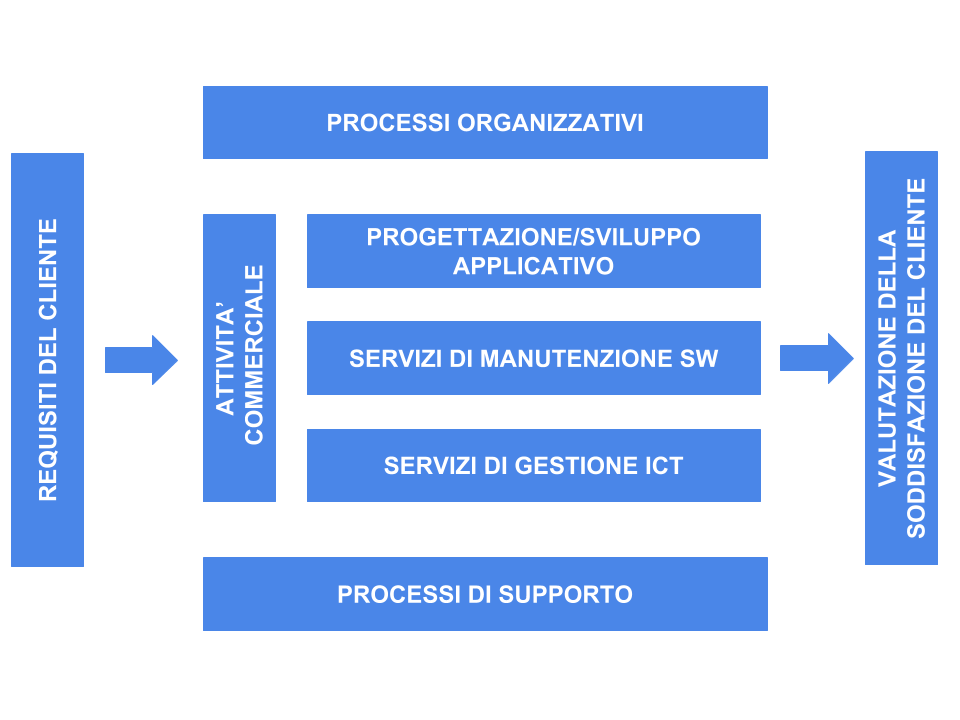
\includegraphics[height=7cm]{relazione-responsabilita}
		\caption{Rappresentazione grafica del coinvolgimento del 
		Cliente e i corrispettivi livelli degli interventi del gruppo 
		commerciale, tecnico, direzionale e di supporto nella gestione 
		di un'offerta di progetto.}
	\end{center}
\end{figure}


\section{Rapporto con l'innovazione}
L'innovazione è il processo di gestione dell'intero ciclo di vita di un'idea. 
L'obiettivo è: portare un miglioramento di processo aziendale, di prodotto e/o 
di servizio. Le conseguenze dirette del miglioramento sono: valore aggiunto, per 
l'azienda, in termini di rientro economico e soddisfare un 
bisogno, per il Cliente, in modo efficace ed efficiente. 

L'approccio innovativo induce l'utilizzo dell'informazione, della creatività e 
dello spirito d'iniziativa per raccogliere maggior valore aggiunto dalle risorse a 
disposizione. L'azienda utilizza l'innovazione per soddisfare in modo pro attivo 
le richieste del Cliente. Questo principio è pienamente il linea con la strategia 
di qualità aziendale: \textit{client first}.

La modalità di innovazione di IKS è un approccio incrementale. Inizialmente 
l'azienda cerca di soddisfare i bisogni principali e raggiungere il prima 
possibile gli obiettivi minimi pre-fissati. In seguito, l'azienda migliora 
la propria offerta mediante incrementi continuativi di dettaglio. 

Per supportare l'innovazione, IKS ha creato una cultura aziendale che permette 
ai propri dipendenti di scambiarsi idee, sperimentare, imparare in gruppo e mettere in 
atto la propria creatività. Non manca la comunicazione con i propri responsabili. 
Questi sono i primi a motivare di continuo le risorse umane a loro disposizione. 
Il dialogo dipendente-responsabile non è verticale. La cultura aziendale in questa 
direzione è molto drastica: favorire uno scambio di idee in modo che esso sia  
equo, semplice e non orientato alle gerarchie aziendali. 

In questo contesto, per l'intera durata del mio periodo di stage e dopo un 
primo momento di ambientamento, io ho beneficiato molto del clima aziendale. 
Infatti, non è mancato il libero confronto con il tutor aziendale, il quale ha  
mostrato disponibilità e apertura al mio spirito d'iniziativa. Sempre mio tutor 
aziendale ha supportato me in ogni scelta decisionale che io abbia motivato e 
ritenuto significativa per il beneficio del mio progetto. 

Le idee sono una parte del processo di gestione dell'innovazione: la realtà è 
molto più complessa. IKS non possiede un effettivo processo di gestione a 
livello aziendale. Questo viene gestito da un gruppo di persone con competenze 
trasversali e a livelli organizzativi differenti. 

\begin{figure}[htbp]
   \begin{center}
	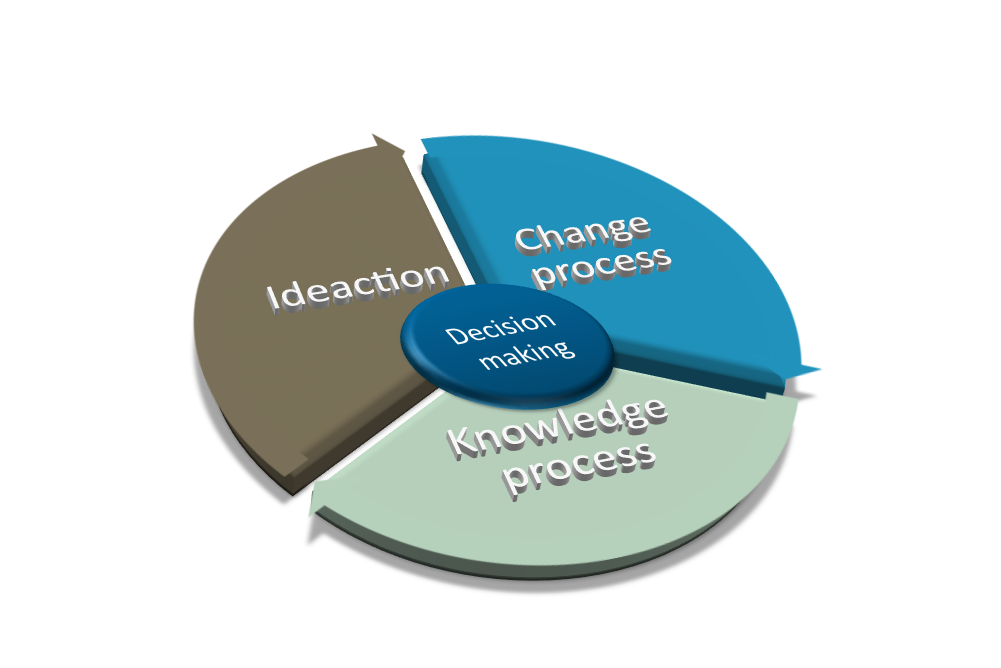
\includegraphics[height=5cm]{innovation-management}
	\caption{Il legame attivo tra innovazione e il processo del cambiamento 
	e gestione della conoscenza. Immagine tratta da: http://bit.ly/2qty3XD.}
   \end{center}
\end{figure}

\newpage              
% !TEX encoding = UTF-8
% !TEX TS-program = pdflatex
% !TEX root = ../tesi.tex
% !TEX spellcheck = it-IT

%**************************************************************
\chapter{L'azienda e gli stage}
\label{cap:stage}
%**************************************************************
\vspace{20pt}
L'azienda investe costantemente sui propri dipendenti per soddisfare 
i bisogni tecnologici del mercato con le giuste competenze. 
I dipendenti dell'azienda dedicano parte della propria giornata lavorativa 
in approfondimenti personali e attività di formazione. 

A supporto dell'attività di laboratorio, il team IT interno ha installato 
un ambiente virtuale. Disporre in azienda di un simile environment permette 
ai dipendenti di sperimentare con: tecnologie, integrazione di sistemi ed ecc. 
Inoltre, offre un'infrastruttura dedicata per i progetti di stage. I temi 
comuni di sperimentazione sono, invece, il  \textit{Cloud}, 
\textit{Machine Learning} e \textit{Analytics}. 

Di recente, l'Azienda ha concluso una partnership strategica con AWS 
(\textit{Amazon Web Services}). Quest'accordo, di collaborazione, 
permetterà a IKS di migrare verso il Cloud e beneficiare delle sue 
peculiarità, per esempio: elasticità, alta affidabilità, flessibilità 
nella gestione di infrastrutture ed ecc. 

Ogni anno, l'azienda partecipa a StageIT: un evento completamente dedicato 
agli studenti universitari dei Corsi di Laurea in Scienze e Ingegneria 
Informatica.
Infatti, StageIT permette  allo studente di mettersi in contatto diretto 
con le aziende e queste ultime di promuovere i propri progetti di stage. 
L'evento prevede, inoltre, un concorso per premiare il miglior progetto 
di stage svolto nell'edizione precedente. Il vincitore del concorso, 
scelto dagli studenti, ottiene come premio un buono d'acquisto del 
valore di 500 Euro.

\section{Il valore aggiunto di uno stagista}

IKS è un partecipante attivo a StageIT; annualmente l'azienda propone 
fino a 6 progetti di stage. Gli argomenti degli stage non sono verticali 
su un'unica tematica, ma coinvolgono temi come: 

\begin{itemize}
	\item Sviluppo di applicazioni basate su web, \gls{cloud}, mobile 
	      o migrazione su \gls{cloud}/mobile di applicazioni tradizionali;
	\item Progettazione di ambienti, metodologie e strumenti di 
	      sviluppo software.
\end{itemize}

Lo stagista è una risorsa importante per IKS; esso porta idee nuove e 
contribuisce a consolidare il valore aggiunto aziendale.
In principio, l'azienda impiega lo stagista su progetti di sperimentazione. 
Questi ultimi hanno come obiettivo l'analisi di fattibilità e lo studio 
dell'integrazione delle soluzioni nell'offerta commerciale dell'azienda. 

Per l'intera durata dello stage, lo stagista opera in un ambiente vero 
simile alla realtà aziendale. Il tutor esterno, oltre a guidare nel lavoro 
lo stagista in relazione a un PdL (Piano di Lavoro), osserva le attività 
dello stagista. 
Le osservazioni contribuiscono alla valutazione finale dell'attività di 
stage del tirocinante.

L'Azienda, con il contributo degli stagisti, allinea se stessa con i 
temi di ricerca universitari e con le tendenze tecnologiche del momento 
sul mercato internazionale.

\section{Alcuni temi di stage}
\subsection{AIOps e Machine Learning}
Il progetto di stage tratta l'integrazione del \textit{Machine Learning} 
con strumenti di Application Performance Monitoring. L'obiettivo dello 
stage è sperimentare integrando diverse soluzioni in questo ambito e 
studiarne il prodotto finale. Una conseguenza critica di questo progetto è 
lo sviluppo di un pensiero critico per affrontare le più difficili sfide 
del monitoraggio di applicazioni e infrastrutture. 

Il presente progetto si colloca nell'ambito del 
\textit{application and performance monitoring} che è un 
servizio offerto dall'azienda al supporto della governance IT. 


\subsection{DevOps Automazione}
L'automazione è fondamento di ogni realtà aziendale contemporanea. Infatti, 
il numero di macchine da gestire spesso non è piccolo. Per semplificare i 
compiti di gestione si devono utilizzare strumenti di configurazione e 
automazione. Queste tecnologie permettono di automatizzare tutte le operazioni 
manuali che un sistemista spesso compie durante le attività di manutenzione 
giornaliere. L'obiettivo di questo progetto è l'integrazione di alcuni 
strumenti che semplificano il \gls{patching} dei server e sperimentare con 
nuove tecnologie del settore.
Il presente progetto si colloca nell'ambito del \textit{system management}. 

\subsection{Sviluppo moduli evolutivi in ambito antifrode}
IKS ha grande esperienza in ambito della sicurezza informatica bancaria. Uno 
dei prodotti risultati di questa esperienza è SMASH. L'obiettivo dello stage è 
estendere il prodotto con qualche funzionalità di monitoraggio di azioni 
sospette. Oltre allo sviluppo di moduli evolutivi lo stagista ha la possibilità 
di apprendere delle competenze forti nell'ambito della 
sicurezza informatica. 
La presente proposta di stage è un progetto inter business unit dell'azienda. 
Esso si colloca nell'ambito dello sviluppo di prodotti software e della 
sicurezza informatica nel settore bancario.


\section{Il progetto proposto}
\subsection{Motivazioni}

E' sempre più comune, nelle realtà aziendali, l'approccio agile. 
Quest'approccio 
promuove la comunicazione e concentra l'attenzione di tutti i stakeholder sul 
valore 
finale di prodotto e/o strategia da raggiungere. 

Se gli sviluppatori hanno come obiettivo primario lo sviluppo di un prodotto 
software 
allora i professionisti dell'IT hanno come priorità la garanzia di servizio e 
manutenzione 
periodica del prodotto software realizzato. 

\begin{figure}[htbp]
	\begin{center}
		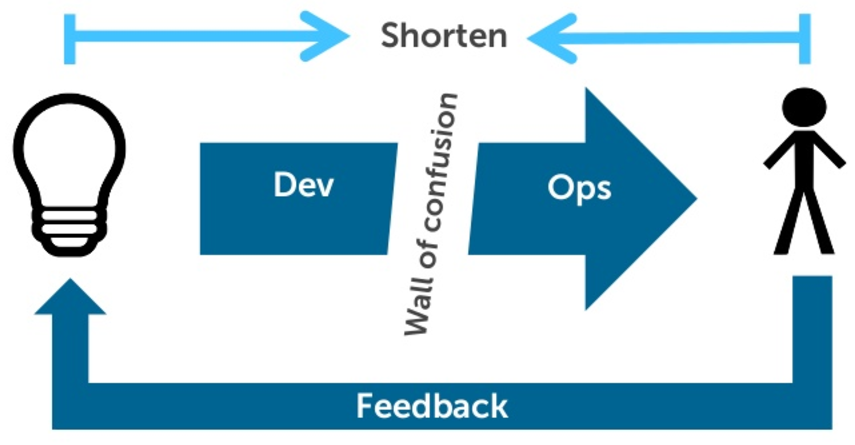
\includegraphics[height=4cm]{devops-wc}
		\caption{Sia gli sviluppatori che i professionisti IT sono 
portatori di valore: 
	    un feedback che coinvolge ambe le parti è essenziale. Immagine 
tratta 
		da: http://bit.ly/2rM9lBQ.}
	\end{center}
\end{figure}


Tra i due gruppi esiste un muro di incomprensione. La mancanza di comunicazione 
ed 
interazione rafforza questo fenomeno. Le problematiche, che avvengono dopo il 
rilascio del prodotto 
software, sono responsabilità dei professionisti IT. Di conseguenza, le loro 
attività 
sono orientate alla risoluzione dei problemi. Una simile organizzazione della 
distribuzione 
delle responsabilità è normale in contesti di realtà aziendali con rilasci 
sporadici.  

Un'azienda informatica, che deve affrontare un numero elevato di rilasci 
giornalieri, 
necessita di un approccio diverso. A questo scopo il movimento culturale, 
chiamato DevOps, è orientato all'unione degli sviluppatori e sistemisti. 
L'unione promuove un cambio di mentalità, creazione di nuove competenze e 
sviluppo di nuovi strumenti che diminuiscano la distanza tra le due realtà. 

Il DevOps ha conseguenze più profonde del semplice cambio culturale.  
Esso introduce un cambiamento interno orientato alla modifica del modello 
di qualità. I benefici di questo cambiamento sono i seguenti: maggiore 
innovazione, qualità di prodotto, processo e agilità nel cogliere i bisogni di 
mercato del momento.

Una tipica rappresentazione del ciclo di vita DevOps segue in figura. 

\begin{figure}[htbp]
	\begin{center}
		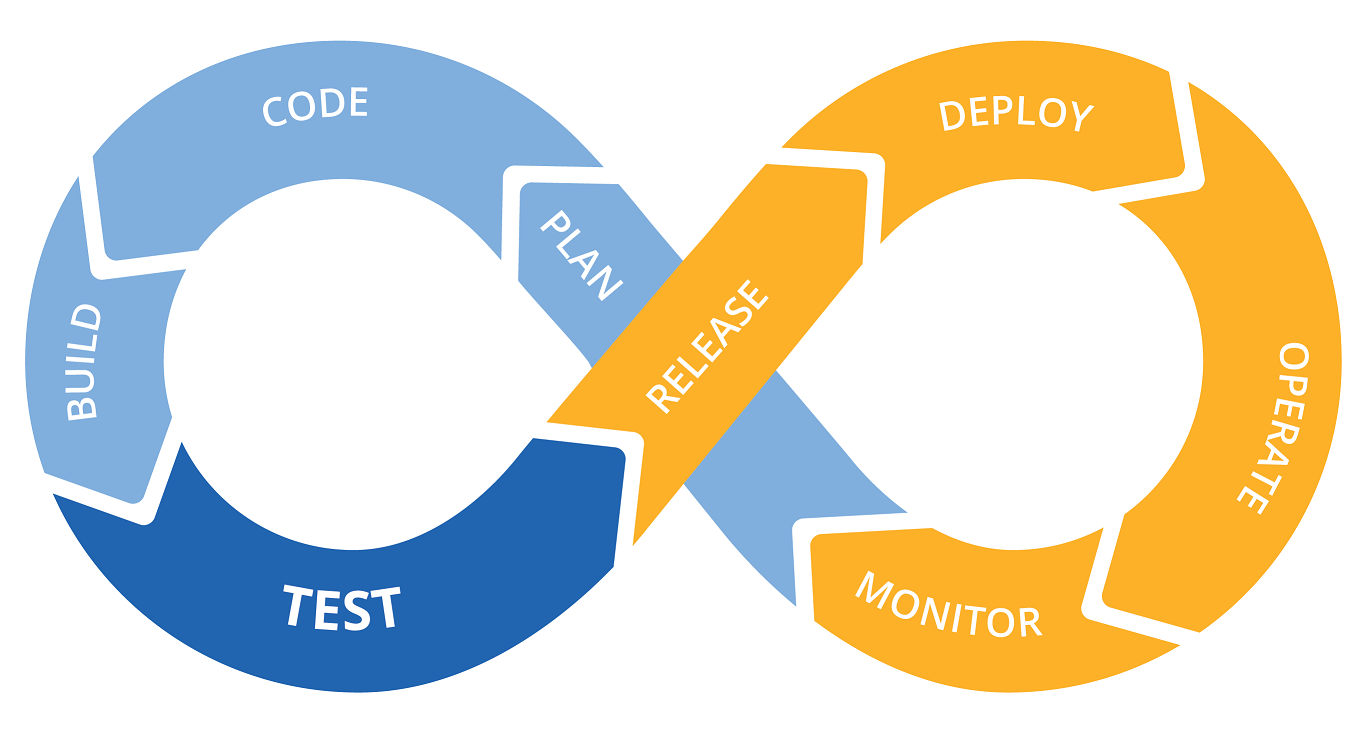
\includegraphics[height=4cm]{devops-pipeline}
		\caption{Il DevOps abilita l'automazione del processo di 
rilascio del software e i cambi dell'infrastruttura IT. Immagine tratta da: 
http://bit.ly/2rsw9nm.}
	\end{center}
\end{figure}

L'abilità di cambiare in modo agile è un grande beneficio per le aziende: il 
modo di lavorare diventa più flessibile e i dipendenti mostrano un maggior 
coinvolgimento nella quotidianità aziendale.    

Lato infrastrutturale, invece, la gestione diventa: disciplinata, sistematica e 
standardizzata. Con un approccio standardizzato e ben strumentalizzato è sempre 
più difficile individuare server nomadi. Può succedere che, in caso di 
operazioni sofisticate e mirate alla manutenzione, un server scompaia 
dall'orizzonte di visibilità. In assenza di opportuni strumenti è difficile 
individuare l'accaduto.   

Sebbene il DevOps possieda uno scopo più ampio, il \textit{continuous delivery} 
è un approccio che promuove l'automazione di tutti i processi coinvolti 
durante il rilascio di un prodotto software. Questo permette di abbreviare i 
tempi, aumentare il numero dei rilasci e migliorare la gestione del cambiamento.

Essere veloci nel \textit{delivery} di un prodotto software non è sufficiente. 
E' importante prevedere una \textit{pipeline} di \textit{deployment} che 
coinvolga ogni \textit{stage} del ciclo di \textit{operation}. Automatizzare il 
\textit{deployment} implica minor intervento manuale, minor numero di errori e 
conseguentemente maggiore formalità nelle attività complessive coinvolte. 

Un \textit{application container} permette di confezionare le applicazioni e 
dipendenze esterne in unità singole. Implementare il \textit{packaging} in 
questo modo le applicazioni facilita lo scambio di artefatti tra tutti i gruppi 
coinvolti nel ciclo di vita del prodotto software. Di conseguenza; sia il 
professionista IT che lo sviluppatore instaurano un protocollo di comunicazione 
e scambio di esperienze basato su qualcosa di concreto, stabile e funzionante.
Il classico detto "funziona sul mio computer" perde di significato.

Al momento la comunità open source offre molte tecnologie di 
containerizzazione. Quella più stabile e famosa nel comunità Linux è LXC 
(\textit{Linux Kernel Container}); questa tecnologia aggiunge il supporto a 
livello del kernel dei container applicativi per i sistemi operativi Linux. 
Docker, invece, è un'altra soluzione di containerizzazione. Le prime versioni 
di Docker interagivano con LXC; le versioni recenti di Docker hanno rimosso la 
dipendenza software verso LXC e ha implementato una soluzione di 
containerizzazione proprietaria. 

La containerizzazione è una tecnologia molto attraente. Visti i vantaggi 
tecnici, la containerizzazione porta a un livello superiore il modello 
concettuale rappresentante un'applicazione.  L'architettura dei prodotti 
software, dal punto di vista dei container, risulta essere più componibile. In 
un ambiente dinamico, caratterizzato dall'automazione, verifiche e 
\textit{deployment} automatici, le classiche architetture software non sono 
pensate per beneficiare di questa flessibilità. Lo stesso non vale per i  
microservizi. 

I microservizi rappresentano uno stile architetturale in sintonia con la 
filosofia Unix: ogni microservizio implementa una sola funzionalità - basso 
accoppiamento.

\begin{figure}[htbp]
	\begin{center}
		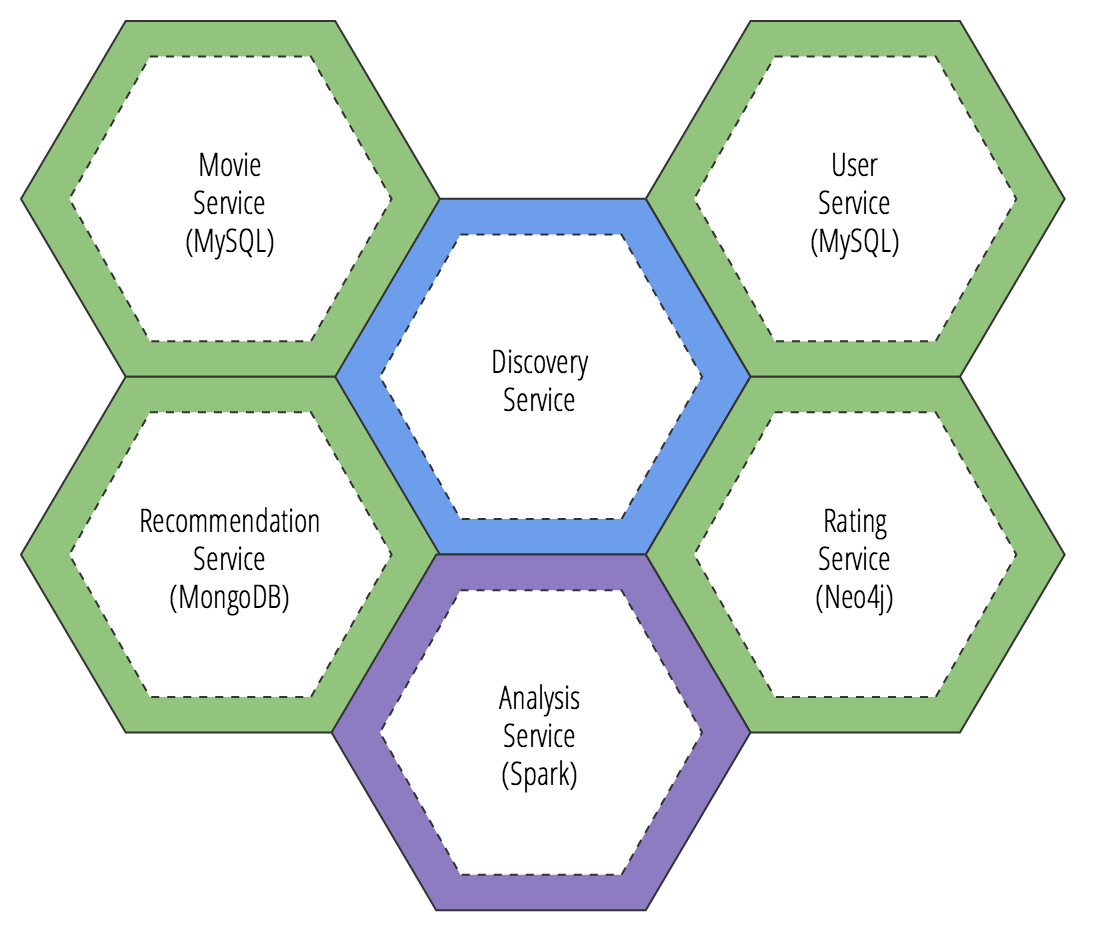
\includegraphics[height=5cm]{microservice-example}
		\caption{Esempio di un sistema a microservizi. Immagine tratta 
da: http://bit.ly/2qNXKxj.}
	\end{center}
\end{figure}

La figura presenta graficamente diversi microservizi. Ciascuno dei quali ha una 
responsabilità ben definita. Per garantire un basso accoppiamento tra i 
microservizi, il sistema deve utilizzare un servizio infrastrutturale e di 
supporto, chiamato \textit{Service Discovery}, utilizzato come un DNS 
(\textit{Domain Name System}). In questo modo, i microservizi continuano ad 
essere autonomi, mentre la gestione della comunicazione inter microservizio è 
separata dall'evoluzione dei singoli microservizi. 
In aggiunta, i microservizi beneficiano della \textit{space transparency}. Se 
un microservizio X, in esecuzione su una macchina A, migra per eseguire su una 
macchina B, allora un microservizio Y, che vuole comunicare con X, deve 
contattare il \textit{Service Discovery} per ottenere l'indirizzo di X. 
L'effetto ottenibile è un alto tasso di mobilità dei servizi.  

E' usuale incapsulare un microservizio in una capsula - il container software. 
Per la proprietà di isolamento: nello stesso ambiente possono coesistere due o 
più copie dello stesso microservizio, riducendo quasi a zero l'interferenza di 
un microservizio su un'altro. 
Con la scalabilità orizzontale i microservizi beneficiano dell'incremento in 
robustezza e alta affidabilità. Per implementare il \textit{routing} delle 
richieste verso i microservizi, i professionisti IT configurano un 
microservizio di \textit{load balancing} a livello applicativo del modello OSI 
(\textit{Open System Interconnection}).


\begin{figure}[htbp]
	\begin{center}
		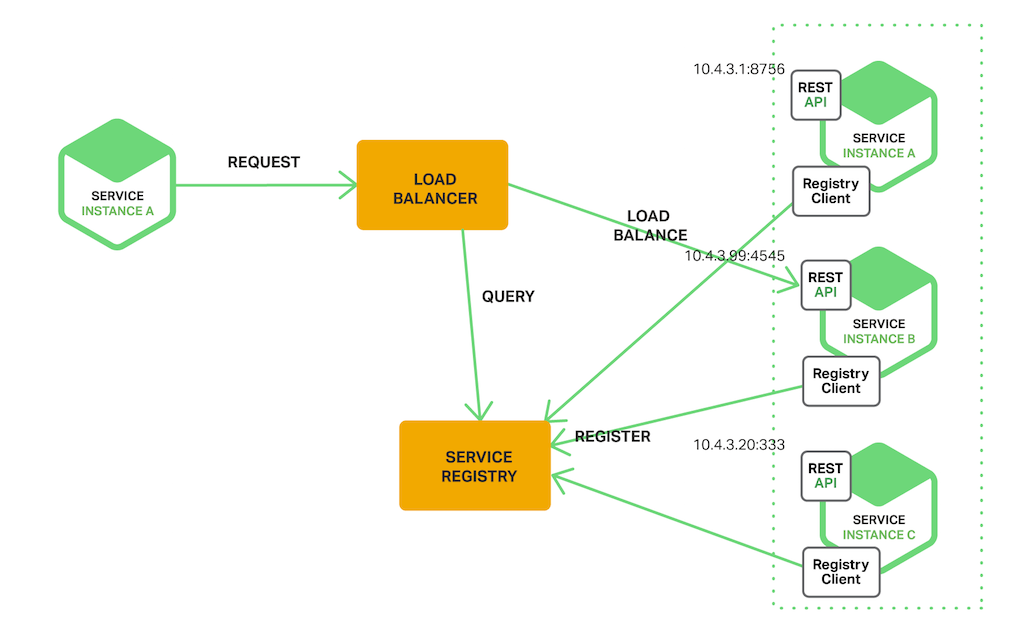
\includegraphics[height=6cm]{richardson-microservices}
		\caption{I microservizi permettono di scalare orizzontalmente 
per reggere ai più esigenti carichi di lavoro. Immagine tratta da: 
http://bit.ly/2qI50LR.}
	\end{center}
\end{figure}

I microservizi semplificano l'analisi, progettazione e implementazione 
dell'applicazione complessiva, scomponendo il prodotto complessivo in sotto 
applicazioni indipendenti; inoltre, i microservizi complicano l'applicazione a 
causa di: un elevato numero di componenti da gestire, difficoltà di versionare 
i microservizi in modo consistente e indipendente, politiche complesse di 
monitoraggio ed ecc. Per la tracciabilità delle richieste inter servizio è 
usuale utilizzare strumenti specializzati nel monitoraggio. Esempi di 
applicazioni, a questo scopo, sono: Appdynamics, Dynatrace, Instana ed ecc. 

I container e microservizi aprono nuove sfide sia per gli sviluppatori che per 
i sistemisti. E queste sfide caratterizzano il contratto di collaborazione tra 
i due gruppi. 


%%% 
------------------------------------------------------------------------------

%%% 
-------------------------------------------------------------------------------

\subsection{Obiettivi aziendali}

Un team interno di IKS ha sviluppato una soluzione di Executive e Malware 
Dashboard
basata sullo stack applicativo: Elasticsearch, Logstash e Kibana.
 
La mia attività di stage ha avuto la containerizzazione della soluzione 
precedentemente implementata come obiettivo principale.

Di seguito presento gli obiettivi principali della mia attività di stage:

\begin{itemize}
	\item Containerizzare le componenti applicative, costituenti la 
soluzione implementata dal team interno di IKS; 
	\item Garantire la non regressione al livello funzionale della 
soluzione;
	\item Predisporre un ambiente containerizzato con e senza orchestratore 
di container.
\end{itemize} 

In conclusione, la containerizzazione garantisce che la soluzione di executive 
e malware dashboard sia portabile su ambienti diversi, dal portatile del 
sviluppatore al Cloud.  

\subsection{Obiettivi personali}
Come attività preliminare alla ricerca di un progetto di stage per la Laurea ho 
attuato uno studio individuale di mercato. Lo scopo era capire: tendenze 
tecnologiche, architetturali e metodologiche. Se da un lato le mie ricerche 
hanno cercato di cogliere le novità del momento, dall'altro a livello personale 
queste erano mirate alla ricerca di un contesto in cui potermi applicare e 
maturare. 

Con il presente progetto gli obiettivi personali erano:

\begin{itemize}
	\item Apprendere conoscenze e competenze in ambito di:
		\begin{itemize}
			\item Virtualizzazione basata sulla tecnologia a 
container; 
			\item Sistemi distribuiti;
			\item Amministrazione di sistema Linux;
	    \end{itemize}
	\item Acquisire esperienza pratica nella gestione delle reti di 
calcolatori in ambito dei sistemi, nello specifico le reti definite in modo 
programmatico per le tecnologie orientate alla containerizzazione; 
	\item Acquisire esperienza nell'analisi, progettazione e 
implementazione di sistemi orientati ai microservizi;
	\item Famigliarizzare con la piattaforma Kubernetes e i principi del 
\gls{cloud}.
\end{itemize} 

\section{Piano di lavoro}
\label{sec:piano-di-lavoro}
L'azienda ha pianificato un piano di lavoro (PdL) per un totale di 300 ore 
complessive. 
Ho consegnato il documento del PdL all'Ufficio degli Stage presso l'Ateneo 
dell'Università di Padova; una seconda copia del PdL ho consegnato al tutor 
interno; l'ultima copia, invece, 
controfirmata dall'ufficio stage dell'Università ho consegnato all'azienda.

Descrivo brevemente di seguito il contenuto del PdL inerente all'insieme delle 
attività svolte:
\begin{itemize}
\item Fase 1 - Formazione  (56 ore)
	\begin{itemize}
		\item Docker: la tecnologia per la containerizzazione;
		\item Kubernetes: la tecnologia per l'orchestrazione;
		\item Elasticsearch, Logstash e Kibana (ELK): lo stack 
applicativo;
		\item Verifiche delle competenze acquisite;
	\end{itemize}
\item Fase 2 - Analisi e progettazione  (56 ore)
	\begin{itemize}
		\item Analisi delle funzionalità della soluzione non 
containerizzata di dashboard;
		\item Analisi delle modalità di containerizzazione delle 
componenti;
		\item Analisi delle modalità di \textit{deployment};
		\item Progettazione delle modalità di verifica della non 
regressione;
		\item Progettazione architetturale della soluzione; 
		\item Progettazione della modalità di \textit{deployment};
		\item Documentazione;
	\end{itemize}
\item Fase 3 - Implementazione  (188 ore)	
	\begin{itemize}
		\item Installazione e configurazione dell'orchestratore;
		\item Implementazione della soluzione in un contesto con e 
senza orchestratore;
		\item Verifica di non regressione;
		\item Documentazione.
	\end{itemize}
\end{itemize}

\section{Vincoli}
\subsection{Vincoli temporali}
Lo stage ha avuto una durata di 8 settimane, per un complessivo di 310 ore di 
lavoro. Ho lavorato a tempo pieno con il seguente orario: 9.00-18.00. Con la 
pausa pranzo di 1 ora dalle 12.30 alle 13.30. Come pianificato nel PdL,  ho 
seguito le attività in ordine seguendo le fasi della pianificazione. Qualche 
volta ho alterato l'ordine delle attività per adattare le esigenze e ridurre 
gli effetti del cambio di contesto.  Infatti, ogni fase ha coinvolto attività 
mirate al raggiungimento di specifici obiettivi. Per maggior dettaglio sul 
contenuto del PdL riferire la \hyperref[sec:piano-di-lavoro]{sezione Piano di 
Lavoro}.

\subsection{Vincoli tecnologici}

Fin dal primo giorno di lavoro l'azienda mi ha fornito un portatile dedicato 
per l'itero periodo di stage. Inoltre, mi è stato vietato di collegare alla 
rete aziendale qualsiasi dispositivo personale. Inoltre, il portatile di lavoro 
non poteva essere portato a casa.
Per comunicare internamente sono stati utilizzati strumenti di messaggistica 
istantanea, come Skype, per comunicazioni informali e la posta elettronica.

Oltre a questo vincolo, a livello tecnologico sono state fissate le seguenti 
tecnologie:

\begin{itemize}
	\item CentOS7: il sistema operativo installato sulle macchine di 
laboratorio. CentOS7 è la versione open source di RHEL7 (Red Hat Enterprise 
Linux versione 7);
	\item Docker: lo strumento che permette in modo estremamente facile la 
creazione, il \textit{deployment} e l'esecuzione di applicazioni utilizzando la 
tecnologia a container. In questo modo l'utente focalizza l'attenzione su 
questioni diverse dall'installazione e configurazione dell'applicazione. 
	L'architettura di Docker segue in figura. 
	
	\begin{figure}[htbp]
		\begin{center}
			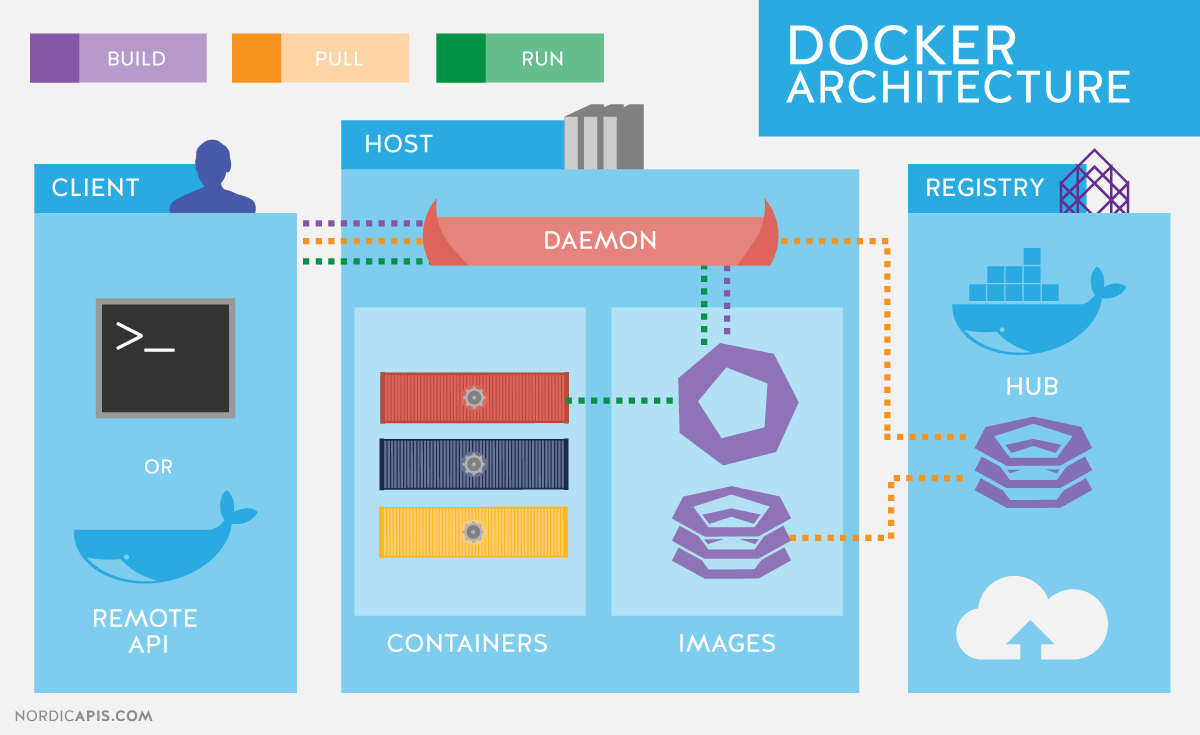
\includegraphics[height=6cm]{docker-architecture}
			\caption{Le parti costituenti la piattaforma Docker 
sono: il demone, il client e il registry Docker. Immagine tratta da: 
http://bit.ly/2rmkt7g.}
		\end{center}
	\end{figure}
	
	Le componenti architetturali costituenti la piattaforma Docker sono il:
	demone, client e registry. L'architettura di alto livello è 
	un architettura client/server. Il server di Docker è il demone che ha 
la responsabilità di gestione dei container sulla macchina locale. Mentre il 
client si interfaccia tramite un'interfaccia REST al demone e permette di 
interagire in modo agile con i container, creare reti virtuali, gestire i dati 
che devono essere condivisi tra i container e il file system locale della 
macchina. Infine, il registry di Docker è una repository che può essere 
pubblica o privata e ha la responsabilità di abilitare la condivisione di 
immagini utili alla creazione dei container. Come modello mentale, in relazione 
con il paradigma ad oggetti, è possibile paragonare le immagini Docker a classi 
che devono essere istanziate per la creazione di oggetti, ovvero container. 
	
	Per favorire il libero scambio di immagini Docker, l'azienda Docker Inc 
ha 
	messo a disposizione degli utenti un hub: spazio web per la 
condivisione delle immagini Docker. Nella modalità privata di una repository, 
Docker Inc rende disponibile 
	il servizio di \textit{scanning} delle vulnerabilità delle immagini. 
	
	Quando l'utente esegue il comando run tramite la CLI di Docker, il 
demone controlla che l'immagine da istanziare, per la creazione del container, 
sia presente sul \textit{file system} locale. In caso affermativo, il demone 
Docker crea e mette in esecuzione il container, altrimenti esso scarica prima 
l'immagine dal registry e al termine, di questa attività, istanzia il container;
	\item Kubernetes: è un sistema open source per automatizzare il 
\textit{deployment}, la scalabilità e gestione di applicazioni containerizzate. 
La tecnologia è il 
	risultato di 15 anni di esperienza in Google con la tecnologia a 
container. 
	Kubernetes garantisce la portabilità delle applicazioni e 
l'indipendenza dall'ambiente fisico di esecuzione.
	
	Kubernetes è un sistema distribuito per l'orchestrazione di container 
applicativi. Il modello architetturale dell'orchestratore è master/slave.
	
	\begin{figure}[htbp]
		\begin{center}
			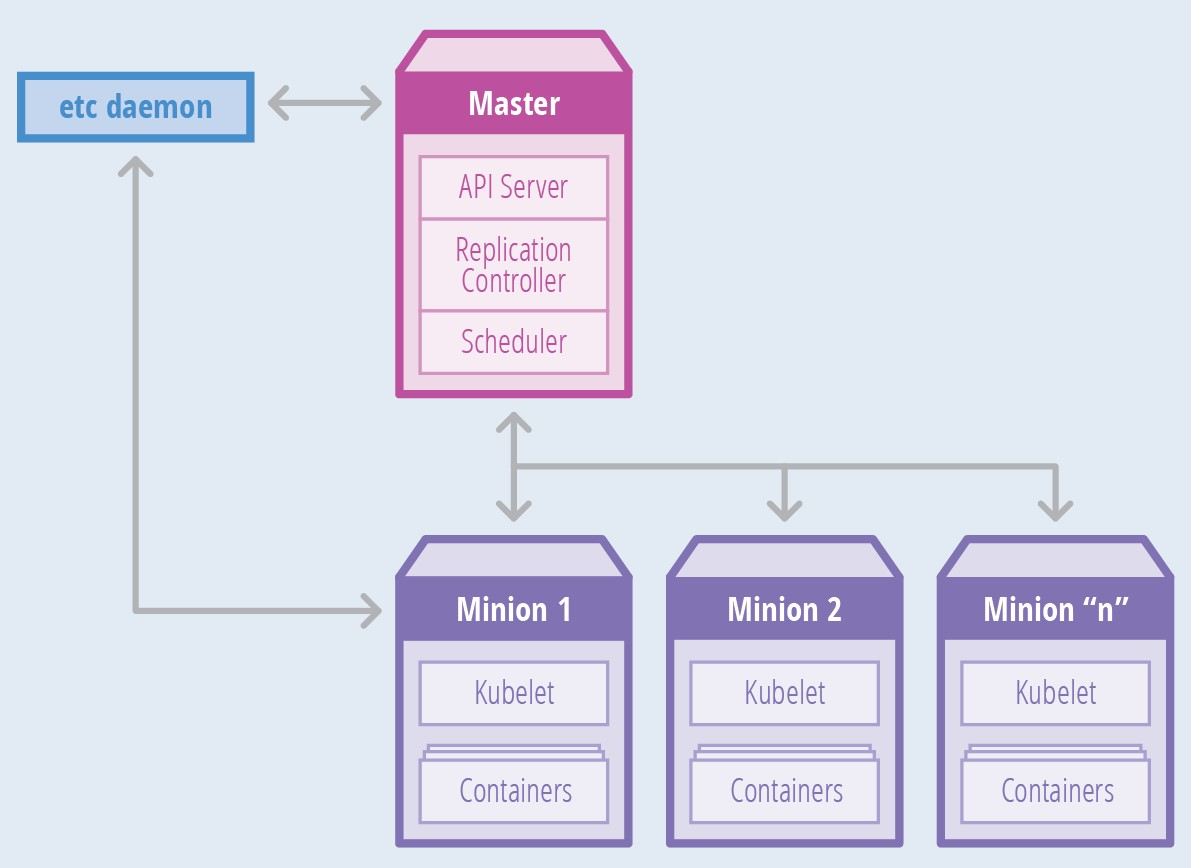
\includegraphics[height=6cm]{kube-architecture}
			\caption{Le componenti architetturali di Kubernetes 
sono: API server, Scheduler, Replication Contoller, Kubelet, Kube proxy, 
Database Etcd. Immagine tratta da: http://bit.ly/2s4eKUR.}
		\end{center}
	\end{figure}
	
	Il master è un pannello di controllo del sistema K8s (Kubernetes). Lui 
gestisce il \textit{workload} dei container. Inoltre, esegue le componenti 
critiche del sistema: il database chiave valore ad alta consistenza 
\textbf{etcd}, il gestore delle repliche per la scalabilità orizzontale - 
\textbf{replication controller} e lo \textbf{scheduler}.  
	
	La componente slave esegue il carico di lavoro. Essa comunica solo con 
il master e salva le informazioni di servizio, tramite il API server, nel 
database etcd. 
	
	Ogni componente master e slave eseguono un agente locale chiamato 
Kubelet. L'agente collega le varie componenti e interagisce con il demone 
Docker. 
	
	Infine, il Kube Proxy è la componente che gestisce il traffico di rete 
dell'intera infrastruttura. 
	
    Kubernetes, essendo un sistema fin dall'inizio pensato per essere 
componibile 
    si può integrare bene con soluzioni di terzi parti, come per esempio: 
diverse soluzioni per lo storage, diversi plugin per la rete ed ecc;
	
	\item Elasticsearch, Logstash e Kibana: Le tre componenti sono 
comunemente conosciute con l'acronimo ELK.  Esse vengono utilizzate insieme 
come una soluzione open source in progetti che hanno forti esigenze di ricerca 
e analisi di dati. Elasctisearch è il cuore dello stack applicativo. Esso è un 
database NoSQL e distribuito implementato in Java. Orientato 
all'immagazzinamento di dati non strutturati, Elasticsearch permette di 
effettuare ricerche complesse impiegando millisecondi contro i secondi 
necessari utilizzando un classico DB SQL.
	
	\begin{figure}[htbp]
		\begin{center}
			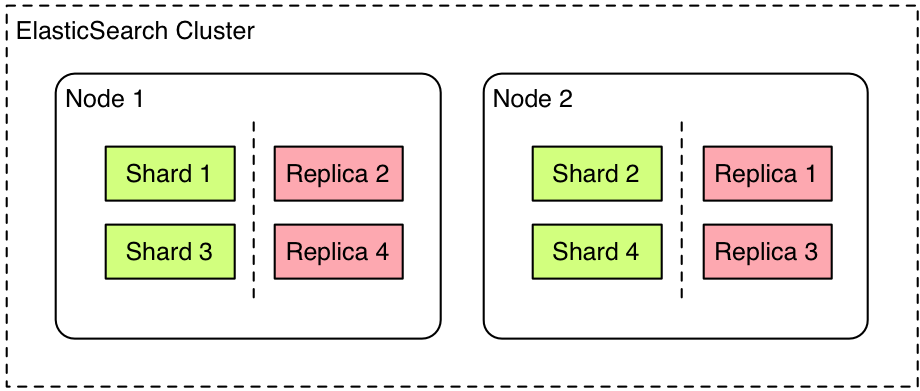
\includegraphics[height=4cm]{es-cluster}
			\caption{Vista di alto livello del meccanismo di 
partizione dei dati immagazzinati in Elasticsearch. Immagine tratta da: 
http://bit.ly/2r0HTQL.}
		\end{center}
	\end{figure}

	Il meccanismo di gestione dei dati di Elasticsearch è complicato. In 
figura è rappresentato un cluster di due nodi. Elasticsearch permette di 
organizzare l'insieme complessivo di dati in sottoinsiemi (\textit{shard}) e 
aggiungere un numero y di copie (\textit{replica}) per ogni sottoinsieme 
primario. Una simile organizzazione permette di garantire un'alta affidabilità 
di dati 
	a livello applicativo. Inoltre, in funzione ai casi d'uso Elasticsearch 
è altamente personalizzabile.
	Per incrementare le performance di lettura, l'utente incrementa il 
numero delle repliche. Per incrementare le performance di scrittura, l'utente 
diminuisce il numero di sottoinsiemi primari dei dati. 	
	Kibana, invece, è la componente dello stack che offre la funzionalità 
di visualizzazione dei dati presenti in Elasticsearch. Una peculiare 
caratteristica di Kibana è l'interfaccia di creazione dei cruscotti. Kibana 
sfrutta l'integrazione nativa con Elasticsearch per esprimere ricerche molto 
complesse e renderizzarle a video tramite effetti grafici accattivanti. Infine, 
Logstash è la componente di estrazione, trasformazione e caricamento dei dati 
dalla sorgente in Elasticsearch. Con Logstash risulta semplice filtrare 
l'informazione utile per l'analisi dei dati ed eliminare il rumore di fondo. La 
comunità open source di Logstash ha sviluppato un insieme molto ricco di 
strumenti che estendono il suo insieme di funzionalità. Per esempio, tramite 
uno plugin esterno è possibile programmare Logstash a interagire con le API 
(Application Program Interface) del social network Twitter, per cercare, 
scaricare e filtrare l'informazione che soddisfa uno specifico criterio di 
ricerca. 
	Dal punto di vista architetturale la soluzione ELK è flessibile e 
permette di scalare facilmente in orizzontale, proporzionalmente al carico di 
lavoro. 
	A seguire allego una rappresentazione grafica delle dipendenze inter 
componenti a livello architetturale. Infatti, Kibana legge da Elasticsearch 
(ES) mentre Logstash scrive in ES.
	
	\begin{figure}[htbp]
		\begin{center}
			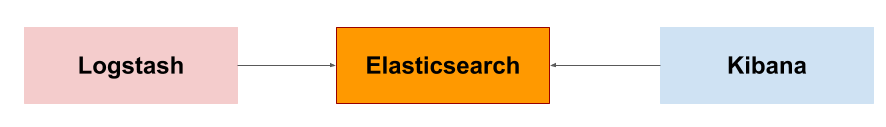
\includegraphics[height=1.5cm]{dipendenze-es}
			\caption{Vista di alto livello del legame sussistente 
inter componente. Il verso della freccia nell'immagine indica una dipendenza.}
		\end{center}
	\end{figure}
	
	  	
\end{itemize}

Inizialmente sono state fissate anche le rispettive versioni delle componenti 
sopra citate. Tuttavia, nel corso dello stage ho realizzato che questo può 
bloccare l'evoluzione dell'infrastruttura e comportare qualche problema in 
futuro. A questo scopo ho predisposto un ambiente tollerante agli 
aggiornamenti. Durante la personalizzazione dell'ambiente mi sono ispirato al 
principio  \textit{self driven infrastructure} di CoreOS. 
In questo modo gli aggiornamenti delle componenti possono essere effettuati in 
modo completamente trasparente.

Infine, come vincolo per le immagini dei container Docker mi hanno imposto di 
utilizzare solo le immagini ufficiali provenienti dal hub di Docker. Questo 
vincolo è dovuto alla presenza di vulnerabilità di sicurezza nelle immagini di 
terzi parti.             
% !TEX encoding = UTF-8
% !TEX TS-program = pdflatex
% !TEX root = ../tesi.tex
% !TEX spellcheck = it-IT

%**************************************************************
\chapter{Lo svolgimento dello stage}
\label{cap:svolgimento-stage}
\vspace{20pt}
%**************************************************************
\section{Metodo di lavoro}

\section{Attività di formazione}

\section{Analisi dei requisiti}
%\subsection{Classificazione dei requisiti}

\subsection{Requisiti}

\subsubsection{Funzionali}

\subsubsection{Non funzionali}


%**************************************************************
\section{Progettazione e realizzazione}

\subsection{Scelte progettuali}

\subsection{Visione architetturale a microservizi}

\subsection{Codifica}

\subsection{Test}

\subsubsection{Test di carico}
\subsubsection{Test di durata}



            
% !TEX encoding = UTF-8
% !TEX TS-program = pdflatex
% !TEX root = ../tesi.tex
% !TEX spellcheck = it-IT

%**************************************************************
\chapter{Valutazioni retrospettive}
\label{cap:valutazioni-retrospettive}
\textbf{TODO: Aggiungere sintesi al capitolo}\\
%**************************************************************

%\intro{Aggiungere abstract}\\

\section{Obiettivi raggiunti}

\section{Problematiche riscontrate}

\section{Bilancio formativo}
\subsection{Il prima}
\subsection{Il dopo}

\section{Valutazione critica del Corso di Laurea}



\newpage
             
%\appendix                               
%% !TEX encoding = UTF-8
% !TEX TS-program = pdflatex
% !TEX root = ../tesi.tex
% !TEX spellcheck = it-IT

%**************************************************************
\chapter{Appendice A}
%**************************************************************
% \epigraph{Citazione}{Autore della citazione}

\section{Machine Learning}

\section{Stile architetturale a microservizi}

\section{Containerizzazione}

\section{Cloud}

             

%**************************************************************
% Materiale finale
%**************************************************************
\backmatter
\printglossaries

% !TEX encoding = UTF-8
% !TEX TS-program = pdflatex
% !TEX root = ../tesi.tex
% !TEX spellcheck = it-IT

%**************************************************************
% Bibliografia
%**************************************************************

\cleardoublepage
\chapter{Riferimenti}

\nocite{*}
%\printbibliography

\bibbycategory % equivale a dare un \printbibliography per ogni categoria


\end{document}